\section{System Model}
\label{sec:system_model}
\begin{figure}[t]
\centering
\resizebox{\linewidth}{!}{%
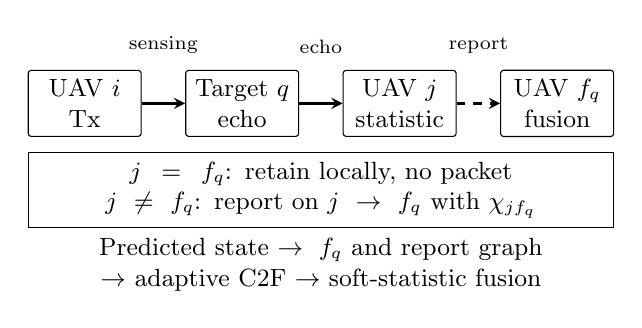
\begin{tikzpicture}[>=stealth, every node/.style={font=\small},
box/.style={draw,rounded corners=1pt,align=center,minimum height=8mm,text width=12mm}]
\node[box] (tx) at (0,0) {UAV $i$\\Tx};
\node[box] (tg) at (2,0) {Target $q$\\echo};
\node[box] (rx) at (4,0) {UAV $j$\\statistic};
\node[box] (fc) at (6,0) {UAV $f_q$\\fusion};
\draw[->,thick] (tx) -- node[above=5mm,font=\scriptsize] {sensing} (tg);
\draw[->,thick] (tg) -- node[above=5mm,font=\scriptsize] {echo} (rx);
\draw[->,thick,dashed] (rx) -- node[above=5mm,font=\scriptsize] {report} (fc);
\node[draw,align=center,text width=72mm] at (3,-1.1)
{$j=f_q$: retain locally, no packet\\
 $j\ne f_q$: report on $j\to f_q$ with $\chi_{jf_q}$};
\node[align=center,text width=72mm] at (3,-2.05)
{Predicted state $\to f_q$ and report graph\\
 $\to$ adaptive C2F $\to$ soft-statistic fusion};
\end{tikzpicture}}
\caption{Sensing and reporting have different endpoints. The fusion UAV is
chosen from predicted target state before observation selection and reporting.}
\label{fig:system_framework}
\end{figure}


\subsection{Task, Prior Information, and Reporting Graph}

Let $\mathcal M=\{1,\ldots,M\}$ and $\mathcal Q=\{1,\ldots,Q\}$ denote
UAVs and targets. Observation $e=(i,j,q)$ is generated at echo receiver $j$:
\begin{equation}
 i\rightarrow q\rightarrow j\rightarrow f_q .
 \label{eq:information_path}
\end{equation}
The sensing pair is $(i,j)$, whereas its reporting link is $(j,f_q)$.
All statistics for target $q$ meet at one fusion UAV $f_q$.
When $j=f_q$, no report is transmitted (Fig.~\ref{fig:system_framework}).

The task is confirmation or re-detection after upstream acquisition.
An external tracker supplies $b_q=\mathcal N(\widehat{\mathbf x}_q,\mathbf P_q)$;
we simulate its output with noisy horizontal position and velocity estimates,
keeping nominal target altitude known. Only this belief and the mean RCS
enter planning. The unknown current state enters echo generation and final
detection. The DD search gate propagates $\mathbf P_q$ through the bistatic
Jacobian and uses three standard deviations per DD coordinate. This gate
models search coverage, not a posterior tracker or blind initial acquisition.

\subsection{Reporting Reliability and Cost}

Sensing and reporting share power, $P_i^{\mathrm s}=\rho P_i$ and
$P_i^{\mathrm c}=(1-\rho)P_i$. The UAV channel gain is
$g_{ab}^{\mathrm c}=(\lambda/4\pi)^2d_{ab}^{-\alpha_{\mathrm c}}
\zeta_{ab}|h_{ab}^{\mathrm c}|^2$, with shadowing $\zeta_{ab}$ and fading
$h_{ab}^{\mathrm c}$. Under orthogonal serial reporting,
\begin{equation}
\begin{aligned}
 \gamma_{ab}^{\mathrm c}&=
 \frac{P_a^{\mathrm c}g_{ab}^{\mathrm c}}
 {N_0+\epsilon_{\mathrm s}\sum_{k\ne a,b}P_k^{\mathrm s}g_{kb}^{\mathrm c}
 +\epsilon_{\mathrm d}P_a^{\mathrm s}g_{ab}^{\mathrm c}},\\
 R_{ab}&=B_{\mathrm c}\log_2(1+\gamma_{ab}^{\mathrm c}).
\end{aligned}
 \label{eq:comm_sinr_rate}
\end{equation}
Here $N_0$ is receiver noise power over $B_{\mathrm c}$, and
$\epsilon_{\mathrm s},\epsilon_{\mathrm d}$ are residual sensing leakage factors.
Reports do not mutually interfere; sensing transmissions remain concurrent.

For a $k$-bit packet in $n$ channel uses, we adopt the normal approximation
for a complex AWGN-equivalent reporting channel~\cite{polyanskiy_fbl}:
\begin{equation}
 \chi_{ab}\simeq1-\mathsf Q\!\left(
 \frac{C(\gamma_{ab}^{\mathrm c})-k/n}
 {\sqrt{V(\gamma_{ab}^{\mathrm c})/n}}\right),
 \label{eq:fbl_reliability}
\end{equation}
where $C(\gamma)=\log_2(1+\gamma)$ and
$V(\gamma)=[1-(1+\gamma)^{-2}](\log_2 e)^2$.
This conditional packet-success approximation replaces the heuristic
$\gamma/(\gamma+\gamma_{\rm req})$; it is not a measured code-specific error curve.
A remote link must satisfy the range mask, $R_{ab}\ge R_{\min}$, and
$\chi_{ab}\ge\chi_{\min}$. Each selected remote observation reserves one
fixed padded $k$-bit report and $n/B_{\mathrm c}$ seconds, without aggregation
or retransmission. Thus $N_{\rm rem}$ reports cost $kN_{\rm rem}$ bits and
$nN_{\rm rem}/B_{\mathrm c}$ serial delay. Local delivery has $\chi=1$ and zero
reporting cost; sensing, processing, and unmodeled control traffic are not free.

\subsection{DD Energy and Local Statistic}

With $\mathbf u_{iq}$ pointing from UAV $i$ to target $q$, the bistatic
coordinates are
\begin{equation}
\begin{aligned}
 \tau_{ijq}&=(d_{iq}+d_{jq})/c,\\
 \nu_{ijq}&=\lambda^{-1}\!\left[(\mathbf v_q-\mathbf v_i)^T\mathbf u_{iq}
 +(\mathbf v_q-\mathbf v_j)^T\mathbf u_{jq}\right].
\end{aligned}
 \label{eq:bistatic_delay_doppler}
\end{equation}
Let $\ell=\tau L\Delta f$ and $\kappa=\nu NT$, with $T=1/\Delta f$.
The coarse estimate is $\eta^{\mathrm c}=\mathrm{sinc}^2(\ell-\mathrm{round}\ell)
\mathrm{sinc}^2(\kappa-\mathrm{round}\kappa)$.
For a periodic $A$-bin axis define
\begin{equation}
\begin{aligned}
 D_A(x)&=\frac{\sin(\pi x)}{A\sin(\pi x/A)},\quad
 p_A(b;z)=\frac{|D_A(b-z)|^2}{\sum_{a=0}^{A-1}|D_A(a-z)|^2},\\
 \eta^{\mathrm{loc}}_{ijq}
 &=\sum_{(b,d)\in\mathcal W_W(\kappa,\ell)}p_N(b;\kappa)p_L(d;\ell).
\end{aligned}
 \label{eq:local_dd_energy}
\end{equation}
The window contains $(2W+1)^2$ bins around the rounded center, with indices
wrapped modulo $(N,L)$. The removable singularity of $D_A$ is evaluated by
continuity. This normalized finite-grid leakage model gives
$0\le\eta^{\mathrm{loc}}\le1$. We use $W=1$ (nine bins) and
$\eta^{\mathrm f}=\eta^{\mathrm{loc}}$, with no interpolation coefficient or gain
floor. The fractional-center cache resolution is $10^{-3}$ bin.
The compact OTFS chain~\cite{hadani_otfs} is checked separately below;
$W=1$ is a fixed processing choice, not a proved optimal window.

With mean target RCS $\bar\sigma_q$,
$g_{ijq}^{\mathrm s}=\lambda^2\bar\sigma_q/[(4\pi)^3d_{iq}^2d_{jq}^2]$,
and
\begin{equation}
 \gamma_{ijq}^{\mathrm s}=
 \frac{P_i^{\mathrm s}g_{ijq}^{\mathrm s}G_{ij}^{\mathrm{hw}}G_{\mathrm p}
 \eta_{ijq}^{\mathrm{DD}}\eta_{ijq}^{\mathrm{col}}}
 {N_0+I_j^{\mathrm s}}.
 \label{eq:sensing_sinr}
\end{equation}
Here $G_{ij}^{\mathrm{hw}}$ contains antenna gains and losses, and $I_j^{\mathrm s}$
includes residual self-interference and concurrent direct paths.
The collision surrogate is $\eta^{\mathrm{col}}=1/n_{ijq}$, where $n_{ijq}$
counts targets in the same rounded DD bin for pair $(i,j)$.
It is an occupancy penalty, not a coherent multi-target interference law.

For $K_{\rm look}$ independent looks, normalized energy $X$ has Gamma shape
$K_{\rm look}$ and scale $1$ under $\mathcal H_0$, or $1+\gamma$ under
$\mathcal H_1$. The centered LLR is
\begin{equation}
 \ell_e=\frac{\gamma}{1+\gamma}(X-K_{\rm look}).
 \label{eq:local_llr}
\end{equation}
Consequently, $\delta_e=K_{\rm look}\gamma^2/(1+\gamma)$,
$v_{e,0}=K_{\rm look}\gamma^2/(1+\gamma)^2$, and
$v_{e,1}=K_{\rm look}\gamma^2$. Look-to-look fluctuation is marginalized by
this energy law rather than sampled again in the mean-RCS link budget.

For successful delivery $A_e\sim\mathrm{Bernoulli}(\chi_e)$, set
$Y_e=A_e\ell_e+(1-A_e)Z_e$, with independent
$Z_e\sim\mathcal N(0,a v_{e,0})$. Total expectation and variance give
\begin{equation}
\begin{aligned}
 \delta_e^{\rm eff}&=\chi_e\delta_e,\\
 \bar v_{e,0}&=[\chi_e+(1-\chi_e)a]v_{e,0},\\
 \bar v_{e,1}&=\chi_ev_{e,1}+(1-\chi_e)av_{e,0}
 +\chi_e(1-\chi_e)\delta_e^2.
\end{aligned}
 \label{eq:received_moments}
\end{equation}
The archived V1 implementation uses $a=9$: failed reports are replaced by
zero-mean uncertainty. This Gaussian replacement is an explicit surrogate,
not a consequence of finite blocklength or a true erasure ($a=0$).
The between-component term in $\bar v_{e,1}$ cannot be omitted.

For independent selected observations, use
$w_e\propto\delta_e^{\rm eff}/\bar v_{e,0}$,
$m_{q,1}=\sum_{e\in\mathcal S_q}w_e\delta_e^{\rm eff}$, and
$v_{q,h}=\sum_{e\in\mathcal S_q}w_e^2\bar v_{e,h}$. The selector predicts
\begin{equation}
\begin{aligned}
 t_q&=\sqrt{v_{q,0}}\left[z_0+\frac{\kappa_{q,0}}6(z_0^2-1)\right],\\
 \widehat P_{D,q}&=\mathsf Q\!\left(\frac{t_q-m_{q,1}}{\sqrt{v_{q,1}}}\right),
\end{aligned}
 \label{eq:detector_prediction}
\end{equation}
where $z_0=\mathsf Q^{-1}(P_{\mathrm{FA}})$ and $\kappa_{q,0}$ is null skewness.
Empty-set prediction is zero. Scheduling uses belief-based moments; final
Monte Carlo detection uses truth-side observations and the same threshold
rule. This remains a moment approximation, not an exact detection probability.
The supplement documents the archived failure-model naming and validation.
